Parámetros del test: \\
Cantidad de iteraciones por filtro 10. Aumentos 100x100.\\
$\alpha = 150$\\
Arrancamos en 1740x60 y vamos aumentando hasta 3840x2160.

\subsubsection*{LDR Y SEPIA}  

\begin{figure}
  \begin{center}
	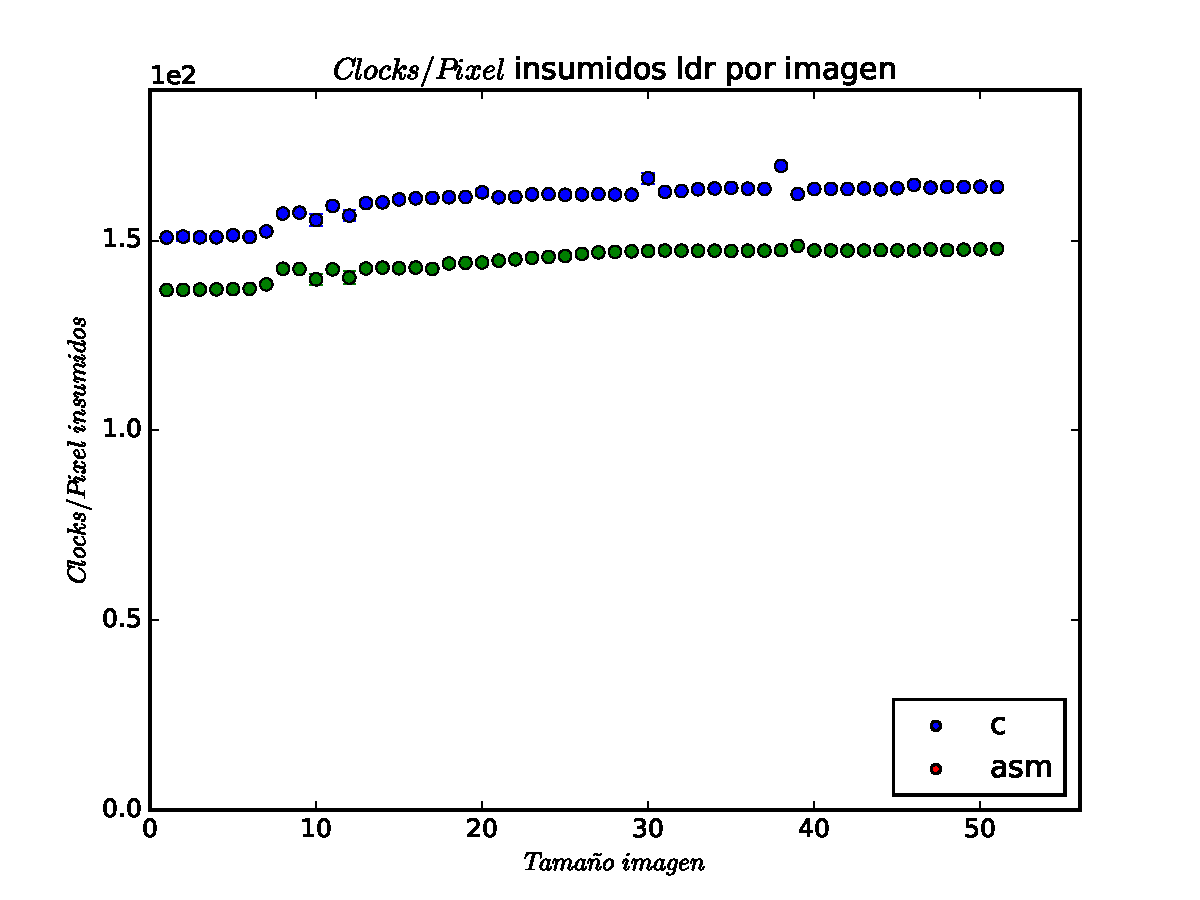
\includegraphics[scale=0.5]{ldrall.pdf}
	%\caption{La última de Star Wars}
  \end{center}
\end{figure}

\begin{figure}
  \begin{center}
	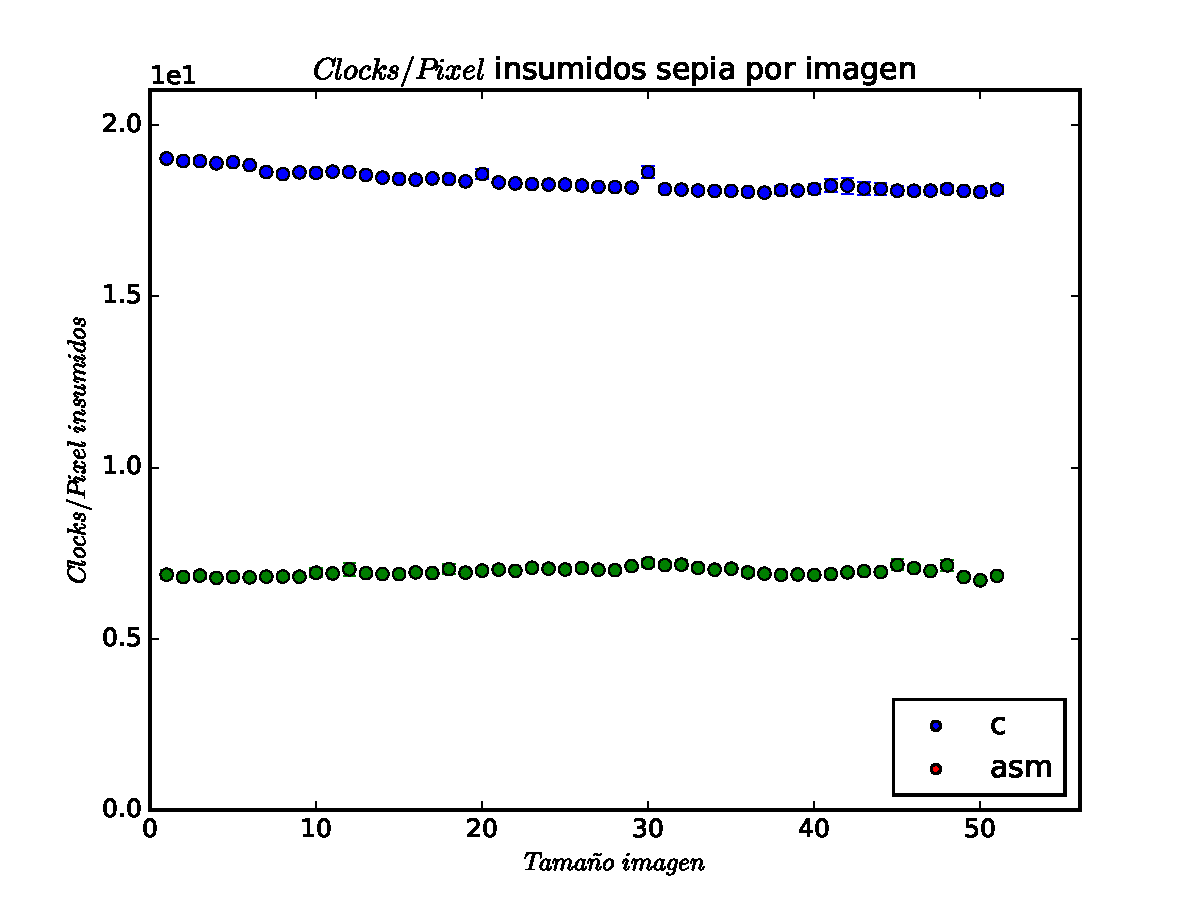
\includegraphics[scale=0.5]{sepiaall.pdf}
	%\caption{La última de Star Wars}
  \end{center}
\end{figure}

Según nuestra hipótesis, con un aumento de forma cuadrática en el tamaño de las imágenes se obtiene una curva casi cuadratica, la curva resultante es muy parecida a una cuadratica pero con un menor crecimiento, en un principio supusimos que esto tenia que ver con que la imagen era mas ancha que alta, asi que invertimos el tamaño de la imágen original de 3840x2160 a 2160x3840 y generamos los mismos aumentos pero invertidos. El resultado obtenido es identico al original, por lo cual no tiene sentido mostrar un gráfico. Suponemos entonces que el factor de anchura o altura de la imágen en estos dos filtros no influye si aumentan los dos en iguales proporciones. \\

\subsubsection*{CROPFLIP}
CORTE: 60 140 0 0 

\begin{figure}
  \begin{center}
	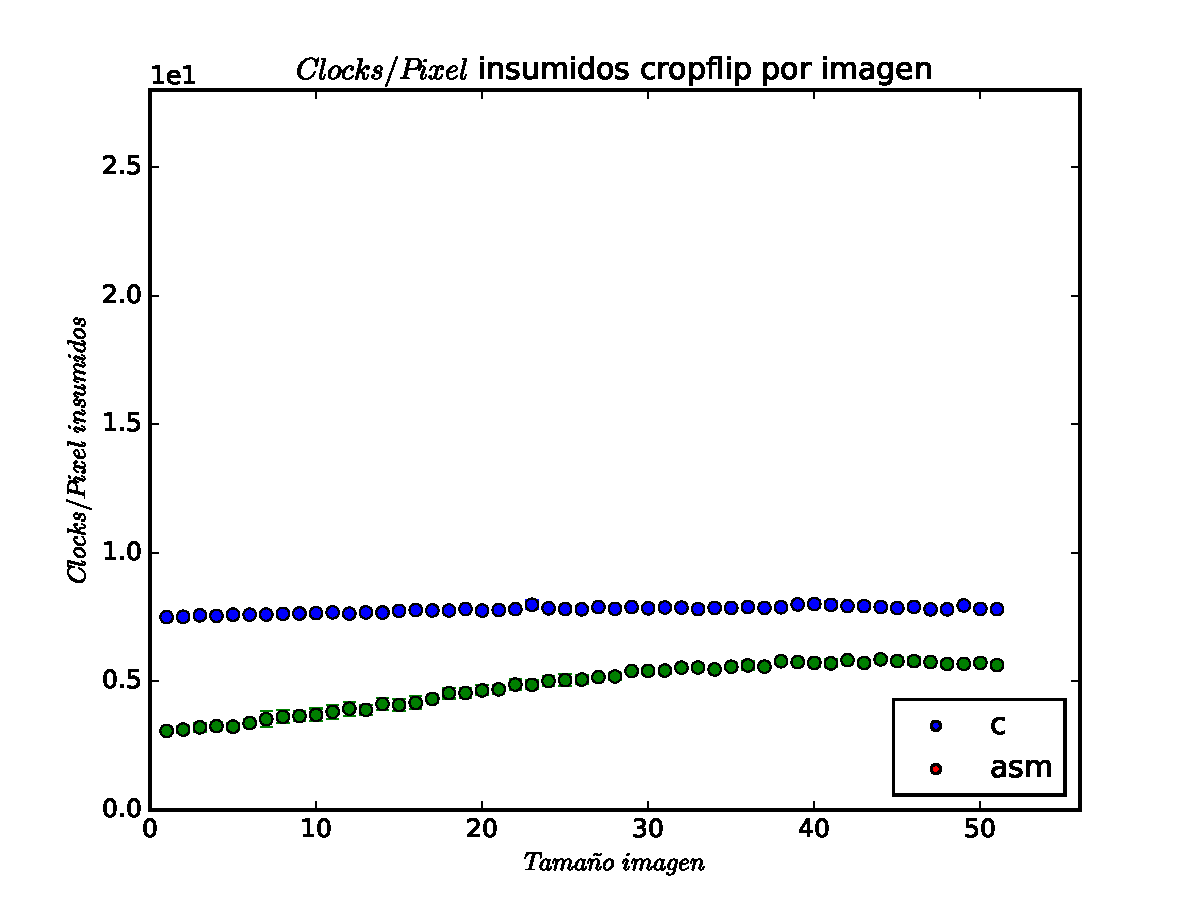
\includegraphics[scale=0.5]{cropflipall.pdf}
	%\caption{La última de Star Wars}
  \end{center}
\end{figure}

Por último observar que en cropflip se mantiene constante, es decir no cumple con lo esperado, (aunque si respeta que assembler es mejor que C). \\

Luego se plantea que con dejar fijo un tamaño y aumentar el otro el resultado seria un aumento lineal de tiempos. Elegimos dejar fija la altura y aumentar el ancho desde 40x2160 a 3840x2160 y el resultado es que si, efectivamente el aumento es lineal. \\

\begin{figure}
  \begin{center}
	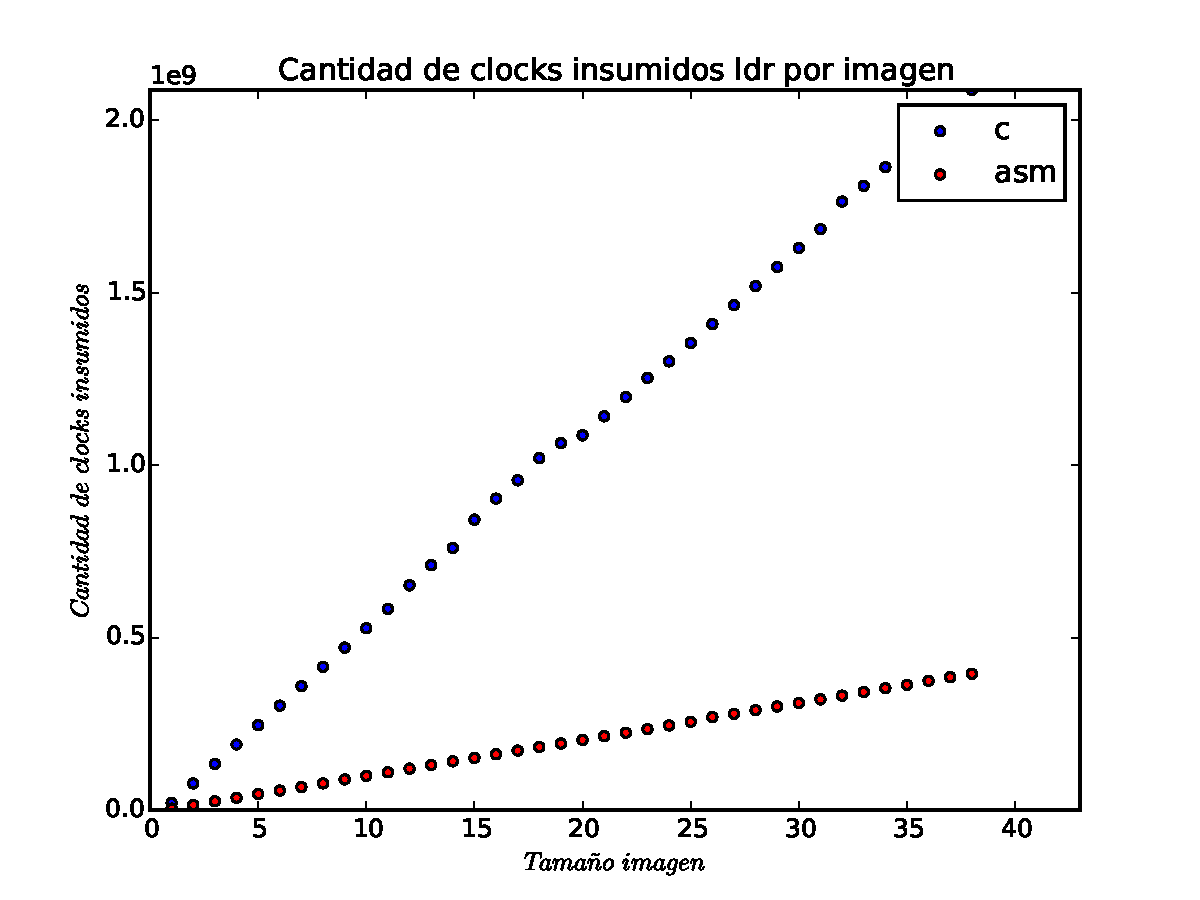
\includegraphics[scale=0.5]{ldrallfijo.pdf}
	%\caption{La última de Star Wars}
  \end{center}
\end{figure}

\begin{figure}
  \begin{center}
	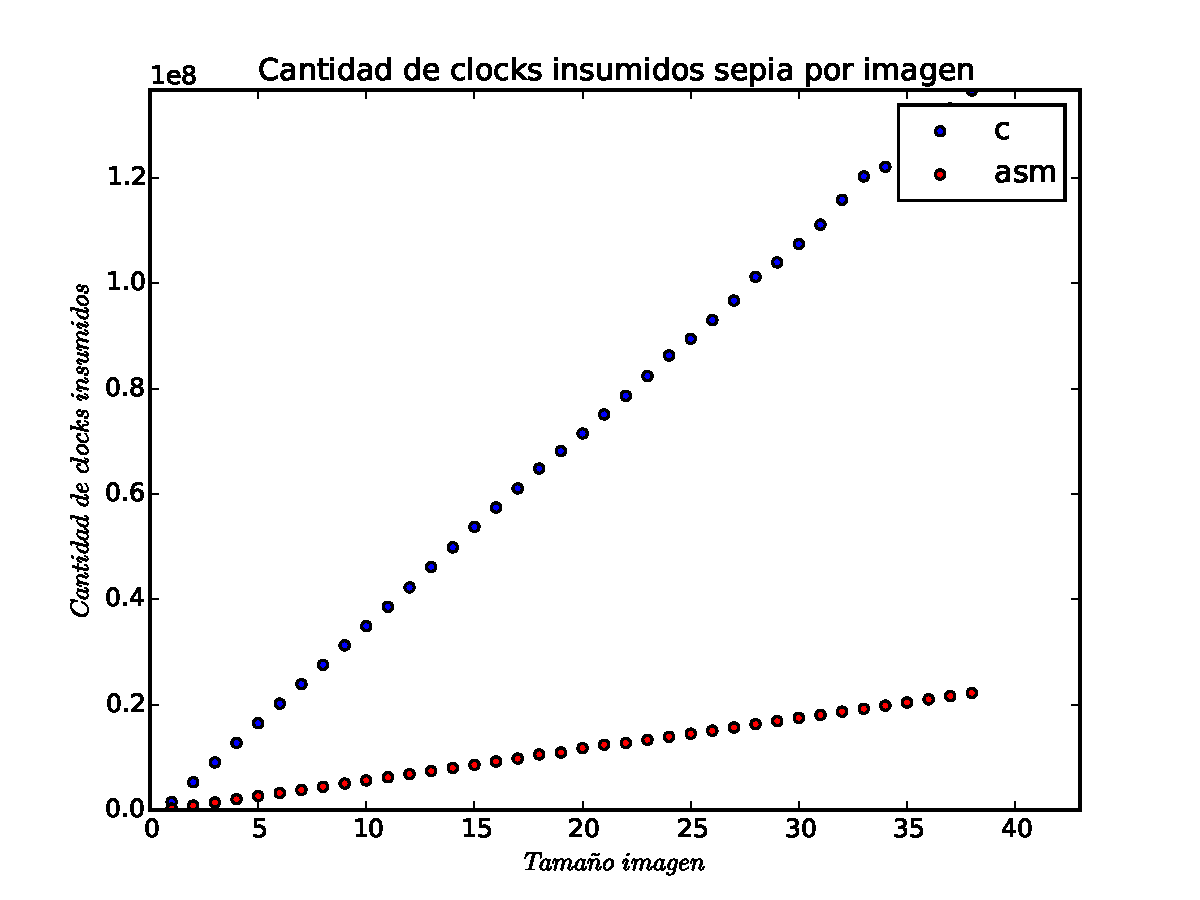
\includegraphics[scale=0.5]{sepiaallfijo.pdf}
	%\caption{La última de Star Wars}
  \end{center}
\end{figure}

\begin{figure}
  \begin{center}
	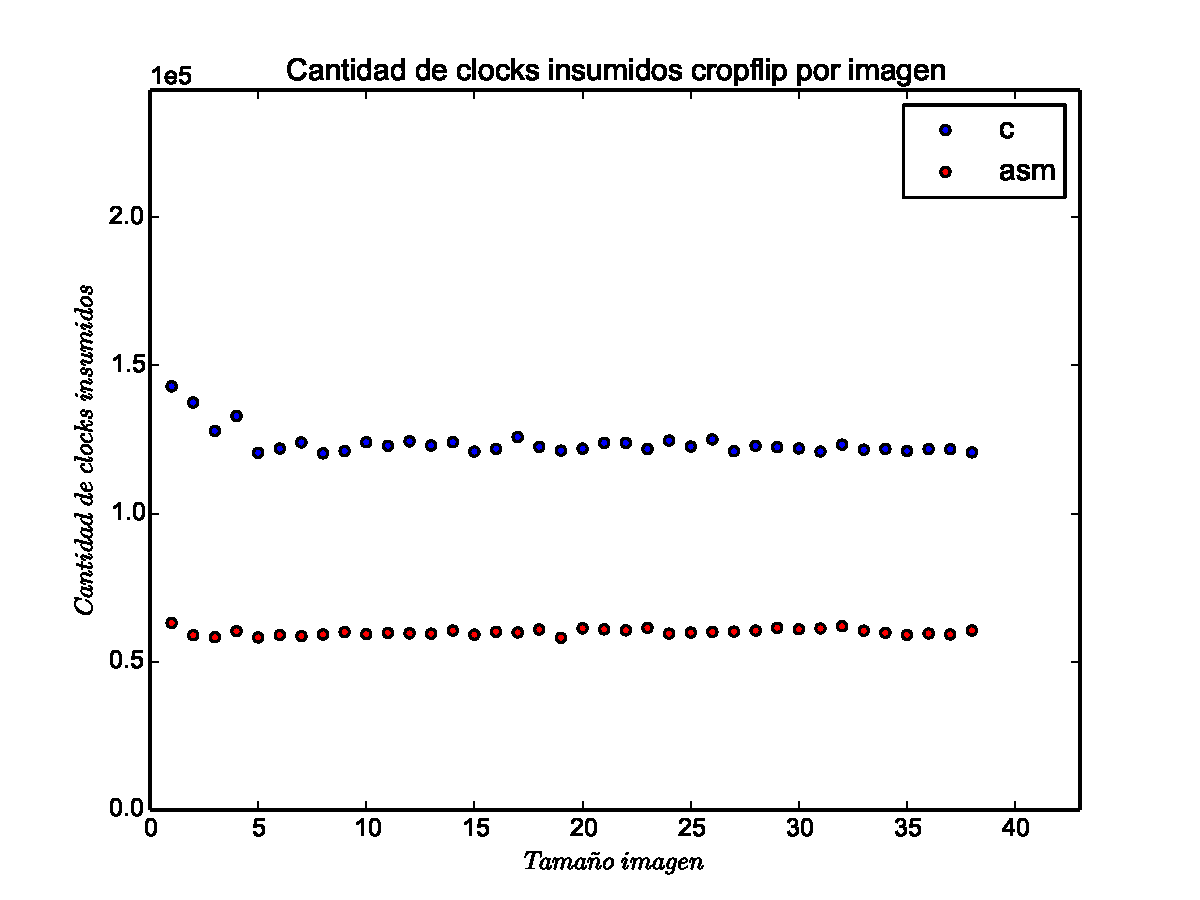
\includegraphics[scale=0.5]{cropflipallfijo.pdf}
	%\caption{La última de Star Wars}
  \end{center}
\end{figure}



